\documentclass[]{article}
\usepackage{amsmath}
\usepackage{amsfonts} 
\usepackage[english]{babel}
\usepackage{amsthm}
\usepackage{mathtools}
\usepackage{subcaption}
\usepackage{hyperref}
\usepackage{algorithmic}
\usepackage{algorithm}
\usepackage{bbm}
% \usepackage{minted}
% Basic Type Settings ----------------------------------------------------------
\usepackage[margin=1in,footskip=0.25in]{geometry}
\linespread{1}  % double spaced or single spaced
\usepackage[fontsize=12pt]{fontsize}
\usepackage{authblk}

\theoremstyle{definition}
\newtheorem{theorem}{Theorem}       % Theorem counter global 
\newtheorem{prop}{Proposition}[section]  % proposition counter is section
\newtheorem{lemma}{Lemma}[subsection]  % lemma counter is subsection
\newtheorem{definition}{Definition}
\newtheorem{remark}{Remark}[subsection]
{
    % \theoremstyle{plain}
    \newtheorem{assumption}{Assumption}
}

\hypersetup{
    colorlinks=true,
    linkcolor=blue,
    filecolor=magenta,
    urlcolor=cyan,
}
\usepackage[final]{graphicx}
\usepackage{listings}
\usepackage{courier}
\lstset{basicstyle=\footnotesize\ttfamily,breaklines=true}
\newcommand{\indep}{\perp \!\!\! \perp}
\usepackage{wrapfig}
\graphicspath{{.}}
\usepackage{fancyvrb}

%%
%% Julia definition (c) 2014 Jubobs
%%
\usepackage[T1]{fontenc}
\usepackage{beramono}
\usepackage[usenames,dvipsnames]{xcolor}
\lstdefinelanguage{Julia}%
  {morekeywords={abstract,break,case,catch,const,continue,do, else, elseif,%
      end, export, false, for, function, immutable, import, importall, if, in,%
      macro, module, otherwise, quote, return, switch, true, try, type, typealias,%
      using, while},%
   sensitive=true,%
   alsoother={$},%
   morecomment=[l]\#,%
   morecomment=[n]{\#=}{=\#},%
   morestring=[s]{"}{"},%
   morestring=[m]{'}{'},%
}[keywords,comments,strings]%
\lstset{%
    language         = Julia,
    basicstyle       = \ttfamily,
    keywordstyle     = \bfseries\color{blue},
    stringstyle      = \color{magenta},
    commentstyle     = \color{ForestGreen},
    showstringspaces = false,
}
\title{Markov Chain Monte Carlo and Simulated Annealing with Applications and Implementations}
\author{Hongda Li}

\begin{document}
\maketitle
\begin{abstract}
    In this report, we prove the fundamentals for the convergence of the Metropolis Hasting Chain under the discrete case; then introduce some ideas from the continuous case. We discuss the Simulated Annealing algorithm as a particular case of the Metropolis Hasting and use both algorithms to construct several numerical experiments in Julia. The first experiment is sampling from complicated distribution functions on 2D, the second is applying Simulated Annealing for the knapsack problem, and in the third experiment, we test simulated Annealing on the Rastrigin function using different base chains. We collect data and illustrate the behaviors of these algorithms. 
\end{abstract}

\numberwithin{equation}{subsection}
\section{Introduction}
    Metropolis Hasting is a Markov Chain Monte Carlo (MCMC) method. It uses the convergence of a Markov chain to sample from a distribution. For motivations, it is easy to sample from a 1D distribution function if we have the inverse of the CDF; however, it is generally tough to sample from a high-dimension distribution even if we have the PDF function. 
    \par
    The Metropolis Hasting Chain (MHC) is a Markov chain whose stationary distribution equals the targeted distribution function. This report is interested in the theoretical foundations for MHC and its applications, and we are also interested in understanding Simulated Annealing (SA) using stochastic processes. 
    \begin{definition}[Stationary distributions]
        Let $p(x, y)$ be a transition kernel for a Markov chain with state space that is countable, then $\pi$ is said to be a stationary distribution for $p$ if it satisfies: 
        \begin{align*}
            \pi(y) = \sum_{x\in S}p(x, y)\pi(x) \quad \forall y \in S. 
        \end{align*}
    \end{definition}
    \begin{definition}[Detailed balance]
        Let $p(x, y)$ be the transition kernel for a Markov chain with state space $S$ which is countable, then the distribution $\pi$ satisfies detailed balance if: 
        \begin{align*}
            \pi(y)p(y, x) = \pi(x)p(x, y) \quad \forall x, y\in S. 
        \end{align*}
    \end{definition}
    \begin{remark}
        If a Markov chain has a distribution that satisfies detailed balance, then the distribution will be the stationary distribution for the Markov chain. 
    \end{remark}
    \begin{definition}[Support of a distribution]
        Let $f$ be a probability mass function with domain $S$, then the support of the PDF is defined as: 
        \begin{align*}
           \text{supp}(f):= \{x\in S: f(x) > 0\}. 
        \end{align*}
    \end{definition}
    

\section{Preliminaries}\label{sec:preliminaries}
    \begin{theorem}[Convergence to stationary distributions]\label{thm:cvg_sta_distr}
        Let $(X_n)_{n\ge 0}$ be a discrete Markov chain with countable/finite state space $S$. Assuming it is irreducible, aperiodic with a stationary distribution $\pi$, then as $n\rightarrow \infty$, we have $p^n(x, y) = \pi(y)$. 
    \end{theorem}
    \begin{proof}
        The theorem is listed as theorem 1.19 in Rick's book \cite{book:rick_essential}. 
    \end{proof}
    \begin{remark}
        This theorem plays a central role in understanding the regularity conditions for the convergence properties of MHC. Moreover, we skip the discussion regarding Markov chains with uncountable state space. For more details about the analysis of the ergodic theorem, see chapter 6 of the book by Robert and Casella \cite{book:robert_casella_2005}. 
    \end{remark}
    \subsection{Metropolis Hasting chain and its convergence}
        In this subsection, we present the proof and theoretical foundations for the convergence of the MHC when the underlying state space is countable. We seek the answer following questions: 
        \begin{itemize}
            \item [1.] What is the MHC? 
            \item [2.] For what regularity conditions can we assert that the stationary distribution is equal to the targeted distribution? 
            \item [3.] What we the regularity conditions imply about the choices of a base chain when it comes to actual applications? 
        \end{itemize}
        We should apply the convergence theorem and analyze the MHC to answer the questions. 
    \subsection{The algorithm}
        The quantities in \hyperref[alg:mhc]{algorithm \ref*{alg:mhc}} has the following quantities and their expectations: 
        \begin{itemize}
            \item [1.] $q(x|y)$ is the base chain defined on $S$ and it has to be doubly stochastic meaning that $q(x|y) = q(y|x)$. 
            \item [2.] $f(x): S \mapsto \mathbb R_+$ is a probability mass function on the state space $S$.
            \item [3.] $\rho$ is the acceptance function, given $X^{(t)}$, it decides whether to accept $Y^{(t + 1)}$ from $q$. 
        \end{itemize}
        \begin{algorithm}
            \begin{algorithmic}[H]
                \STATE{\textbf{Input: $X^{(t)}$}}
                \STATE{$Y^{(t)} \sim q (\cdot | x^{(t)})$}
                \STATE{
                    $
                    X^{(t + 1)} := 
                    \begin{cases}
                        Y^{(t)} & \text{w.p}:  \rho(X^{(t)}, Y^{(t)})
                        \\
                        X^{(t)} &  \text{else}
                    \end{cases}$
                }
                \STATE{
                    $ 
                    \rho(x, y) := 
                    \min\left\lbrace
                        \frac{f(y)}{f(x)}\frac{q(x|y)}{q(y|x)}, 1
                    \right\rbrace
                    $ 
                }
            \end{algorithmic}
            \caption{Metropolis Chain}
            \label{alg:mhc}
        \end{algorithm}
    

    \subsection{Transition kernel of MHC}
        Firstly, the transition kernel of the MHC is given by: 
        \begin{align*}
            K(x, y) = \rho(x, y)q(y|x) + \left(1 - \underbrace{\sum_{y \in S}^{}\rho(x, y)q(y|x)}_{=:r(x)}\right) \mathbbm 1\{y = x\}. 
        \end{align*}
        The above is direct from \hyperref[alg:mhc]{algorithm \ref*{alg:mhc}}. 
        \begin{theorem}[Stationary distribution for the MHC]\label{thm:sat_distr}
            The distribution $f$ satisfies the detailed balance conditions when $x, y\in S$; consequently, the MHC has $f$ as the stationary distribution. 
        \end{theorem}
        \begin{proof}
            Consider any $x, y\in \text{supp}(f)$ with $x\neq y$ then
            \begin{align*}
                \rho(x, y) &= \min\left\lbrace
                \frac{f(y)}{f(x)}\frac{q(x|y)}{q(y|x)}, 1
                \right\rbrace
                \\
                \implies
                \rho(x, y)f(x) &= \min\left\lbrace
                    f(y), f(x)
                \right\rbrace, \rho(y, x) f(y) = 
                \min\left\lbrace
                    f(x), f(y)
                \right\rbrace
                \\
                \implies
                \rho(x, y)f(x) &= \rho(y, x)f(y)
                \\
                \implies
                \rho(x, y)q(y|x)f(x) &= 
                \rho(y, x)q(x|y)f(y)
                \\
                \implies
                K(x, y)f(x) &= K(y, x)f(y), 
            \end{align*}
            when $x = y$, we have $1 - r(x)= 1 - r(y)$, which is just trivial. 
        \end{proof}
        However, the above theorem does not guarantee that the Metropolis chain will converge to the distribution $f$. To converge, it has to be the case that the chain is irreducible on all states in the support set of $f$ (f-irreducible). To be irreducible on the set of $\text{supp}(f)$ means that for all $x, y \in \text{supp}(f), x \rightarrow y$, where $x\rightarrow y$ means that it is possible to commute from the state $x$ to $y$. In general, it is better to judge f-irreducible conditions on a case-by-case basis to determine the choice of the base chain. Nonetheless, the below theorem quantifies a stronger condition to assert the convergence. 
        \begin{theorem}[Regularity conditions for the MHC]\label{thm:reg_cond}
            For a base chain that is non-negative, e.g., $q(x|y) > 0\; \forall x, y\in S\times S$, the MHC is f-irreducible. 
        \end{theorem}
        \begin{proof}
            For all $f(x),f(y)>0$ with $x\neq 0$, we have $q(x|y) > 0$, and since $f(y)/f(x) > 0$, we have $\rho(x,y)$ being non-negative and therefore, it is possible to jump between any state in the support set for $f$. 
        \end{proof}
        \begin{remark}
            Weaker conditions for the regularity conditions exist. For more detail, review Robert and Casella's book \cite{book:robert_casella_2005} in chapters 6 and 7, where it discusses the regularity conditions for the Markov chain with a continuous state space. 
            \par
            In practice, we have to assess the irreducibility on a case-by-case basis for the best choice for the base chain. In most cases, we have no idea what the set $\text{supp}(f)$ even is and how it would be described. 
        \end{remark}
        \begin{theorem}[Convergence of the Metropolis Chain]
            The MHC described in \hyperref[alg:mhc]{algorithm \ref*{alg:mhc}} that satisfies \hyperref[thm:reg_cond]{theorem \ref*{thm:reg_cond}} and has a countable state space will converge to the stationary distributions $\text{supp}(f)$. 
        \end{theorem}
        \begin{proof}
            Observe that MHC in \hyperref[alg:mhc]{algorithm \ref*{alg:mhc}} is aperiodic because there exists $x, y\in \text{supp}(f)$ with $f(x) \neq f(y)$ and therefore allowing $\rho(x, y) < 1$ and giving us none zero probability for rejecting the current candidate. If this is not the case, it has to be $f(x) = f(y)$ for all $x, y \in S$, meaning that the uniform distribution is distribution $f$. In that case, it is the same stationary distribution as the doubly stochastic base chain $q$. 
            \par
            Because it satisfies theorem \ref*{thm:reg_cond} and MHC satisfies \hyperref[thm:sat_distr]{detailed balance (theorem \ref*{thm:sat_distr})}, using \hyperref[thm:cvg_sta_distr]{theorem \ref*{thm:cvg_sta_distr}} MHC will converge to $\text{supp}(f)$. 
        \end{proof}
    \subsection{Numerical experiments}
        In this experiment, we consider sampling from the following functions that we made: 
        \begin{align*}
            D &:= \{(x_1, x_2): -\sin(4\pi x_1) + 2\sin(2\pi x_2)^2 > 1.5\}
            \\
            f(x) &:= \mathbbm 1_D (\sin(x_14\pi) + \cos(x_24\pi) + 2), 
        \end{align*}
        observe that this is not strictly a distribution function, but due to the construction of MHC in algorithm \ref*{alg:mhc}, we have $f(y)/f(x)$, meaning that we can sample any function that is a distribution function up to a constant.
        \par
        For our case, the function $f$ has a discontinuous support set, and the sample space is continuous. Please take for granted that the convergence theorem we proved is applicable for Markov chains with a bounded continuous state space. For our experiment, we will be sampling from $f$ using this list of base chains: 
        \begin{itemize}
            \item [1.] A wrapped Guassian random walks in $[0, 1]\times [0, 1]$ centered at the previous state, or in other words, a guassian random walks with boundary conditions on the domain: $[0, 1]\times[0, 1]$ and the standard deviation for the Gaussian distribution is $0.1$. 
            \item [2.] A uniform distribution in $[0, 1]\times [0, 1]$
        \end{itemize}
        We present the results for both choices of base chain in \hyperref[fig:gaussian_rand_bc]{figure \ref*{fig:gaussian_rand_bc}} and \hyperref[fig:unif_rand_bc]{\ref*{fig:unif_rand_bc}}. We take snapshots of all the existing sampled points every 5000 times. Going from left to right in both cases, we have the approximated distributions when there are 5000, 10000, and 15000 points. These two chains converge very differently for this example, which makes sense. For a uniform random sampler, the previous point does not correlate with the next point from $q$, making it possible to jump between the discrete sets in $\text{supp}(f)$ and sample from them evenly. On the contrary, the Gaussian random walks samplers have difficulties sampling evenly from each of the discrete sets in $\text{supp}(f)$. The argument makes intuitive sense because a Gaussian random walk is more likely to sample from the ``island'' close to the one where the current state resides, and it is nearly impossible for it to jump. This experiment focuses on non-negative double stochastic chain chan $q$; however, it also tells us what happens when the probability of traversing between states in the support set of $f$ when the base chain does not allow for MHC to be f-irreducible. 
        \par
        Finally, the reader should notice that a Monte Carlo method, without the Markov chain, is just sampling using a uniform base chain where the function $f$ is an indicator function for some sets. Moreover, this observation should reveal that MCMC is a type of MC that samples locally. 
        \begin{figure}[H]
            \centering
            \begin{subfigure}{0.3\textwidth}
                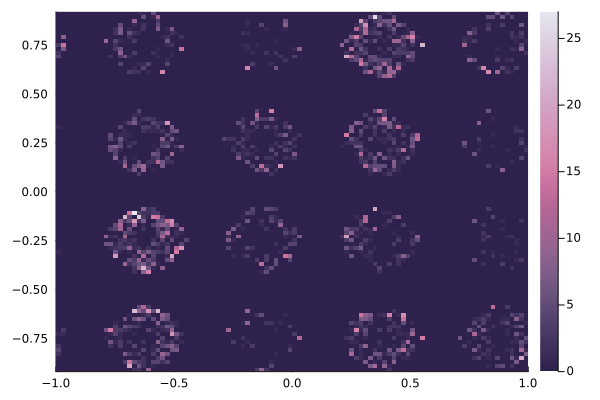
\includegraphics[width=\textwidth]{gaussian_base(1).png}
                \caption{Firt snapshot.}
                % \label{fig:first}
            \end{subfigure}
            \hfill
            \begin{subfigure}{0.3\textwidth}
                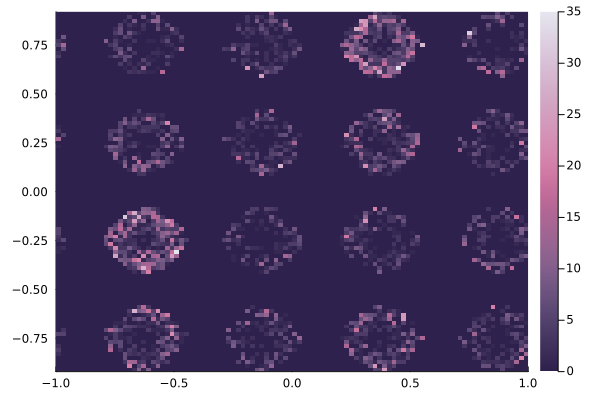
\includegraphics[width=\textwidth]{gaussian_base(2).png}
                \caption{The second snapshot.}
                % \label{fig:second}
            \end{subfigure}
            \hfill
            \begin{subfigure}{0.3\textwidth}
                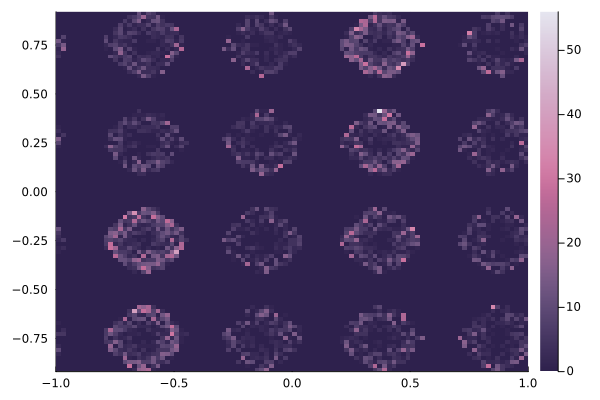
\includegraphics[width=\textwidth]{gaussian_base(3).png}
                \caption{The third snapshot.}
                % \label{fig:third}
            \end{subfigure}
            \caption{Snapshots of accumulated samples when a wrapped Gaussian random walk base chain.}
            \label{fig:gaussian_rand_bc}
        \end{figure}
        \begin{figure}[H]
            \centering
            \begin{subfigure}{0.3\textwidth}
                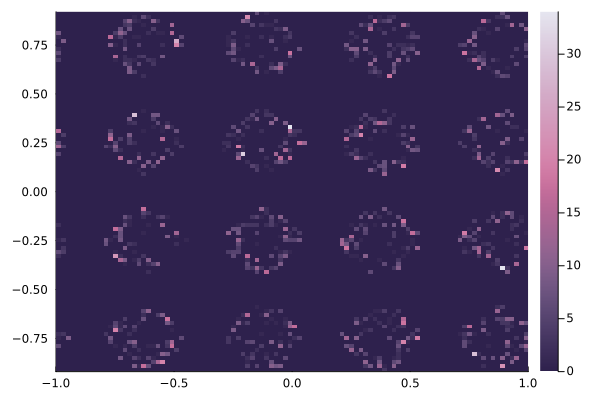
\includegraphics[width=\textwidth]{uniform_base(1).png}
            \end{subfigure}
            \hfill
            \begin{subfigure}{0.3\textwidth}
                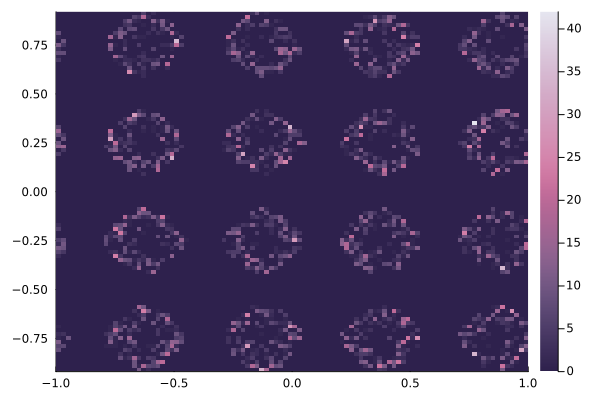
\includegraphics[width=\textwidth]{uniform_base(2).png}    
            \end{subfigure}
            \hfill
            \begin{subfigure}{0.3\textwidth}
                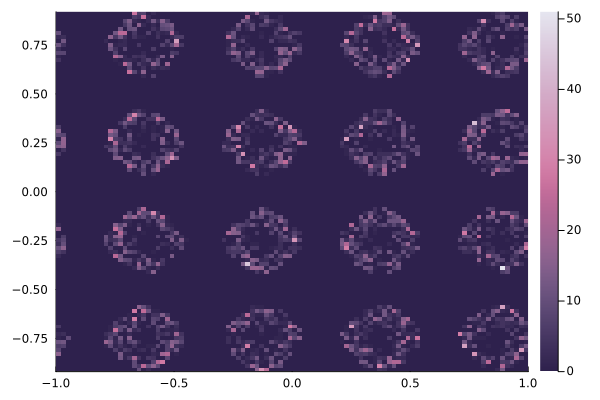
\includegraphics[width=\textwidth]{uniform_base(3).png}                
            \end{subfigure}
            \caption{Snapshot of samples for a uniform random base chain.}
            \label{fig:unif_rand_bc}
        \end{figure}
        As a remark, choosing a base chain is much more complicated in higher dimensions, and using MCMC has overwhelming advantages. As the dimension increases, a unit sphere's volume over the unit hypercube approaches zero. As a result, it poses challenges for sampling from the hypersphere using Monte Carlo. However, if we have an initial point in the hypersphere and a carefully designed base chain, we can sample from a high-dimensional sphere. 

\section{Simulated annealing}
    Simulated Annealing is an optimization method, and it is also a specific case of the MHC. Firstly, observe that if a distribution with a bounded domain and a set $X^*$ in the domain that denotes the maximums and $X^*$ is measurable, then the probability of sampling from $X^*$ is higher than other sets with the same measure. This inspiration here allows us to design and make an optimization method. More specifically, given any function $g:S \mapsto \mathbb R_+ \cup \{-\infty\}$, we have $f(x):= \exp(g(x))$ such that $f$ is a distribution up to a positive constant multiplier. By the monotone property of $\exp(\cdot)$, $f$ and $g$ share the same maximums. 
    \par
    Compared to the MHC, which is about sampling from a distribution, the Simulated Annealing method aims to look for the maximum of a given function and comes with a slight modification called the temperature. The temperature term $T_i$ where $i$ is the current step for the drawn samples from the MHC, we have the distribution function to be given as $f(x):= \exp(g(x)/T_i)$. The goal of the temperature is to accentuate the set $X^*$. The smaller the value $T_i$, the larger the probability it is to sample from the set $X^*$ compare to other sets. 
    \par
    For readers who are optimizations enthusiasts, this is invigorating news. One can see that this method makes few assumptions about the objective function, and there is also a convergence proof for the method \cite{article:sim_anneal_1994}. However, we will show later with the Bin Packing Problem that its performance depends on the problem structure, the base chain, and the temperature schedule. Adding salt to injury, it only converges in distributions. Nonetheless, one can not deny its universality, the fact that it is simple to implement, and it is trivial to parallelize in modern computing platforms. 
    \subsection{The limit of temperature}
        \begin{theorem}[The limit of temperature]
            Suppose that state space $S$ is a finite set, and it is the state space for an MHC equipped with $f(x) = \exp(g(x)/T_i)$ where $g:S \mapsto \mathbb R \cup \{-\infty\}$, then as $T_i\rightarrow 0$, $f$ approaches $\mathbbm 1_{X^*}$. 
        \end{theorem}
        \begin{proof}
            \begin{align*}
                \lim_{i\rightarrow \infty}f(x) 
                &= 
                \lim_{i\rightarrow \infty} \frac{\exp(g(x)/T_i)}
                {
                    \sum_{y\in S}^{}
                    \exp(g(y)/T_i)
                }
                \\
                &= 
                \lim_{i\rightarrow \infty}
                \frac{1}{\sum_{y\in S}^{}\exp(g(y) - g(x)/T_i)}
                \\
                &= 
                \lim_{i\rightarrow \infty}
                \frac{1}{\exp(0) + \sum_{y\in S\setminus\{x\}}^{}\exp(g(y) - g(x)/T_i)}
                \\
                &= 
                \lim_{T\rightarrow 0}
                \frac{1}{1 + \sum_{y\in S\setminus\{x\}}^{}\exp(g(y) - g(x)/T)}
                \\
                &= \mathbbm 1\{X^+\}. 
            \end{align*}
            Take note that the assumption I made here is stronger than it needs to be and might still converge for MHC with a continuous distribution. For more detail about the limiting behavior of the distribution function as $T\rightarrow 0$, see chapter 3 of the book by Levin et al. \cite {book:mkv_mix_time} for more details. 
        \end{proof}
        To illustrate the process of changing temperature, we make an example involving $g(x) = \text{sinc}(x)$ and choose temperatures from $1$ to $10^{-2}$ geometrically distributed. Then we plot the normalized function $f(x):= \exp(\text{sinc}(x)/T_i)$ on the interval $[-3, 3]$ and it produces figure \ref*{fig:sa_temp}. Observe that the function's maximum accentuates as the temperature gets lower, which means that the MHC is more likely to reject states with lower values and climb more aggressively than when the temperature is still high. 
        \begin{figure}[H]
            \centering 
            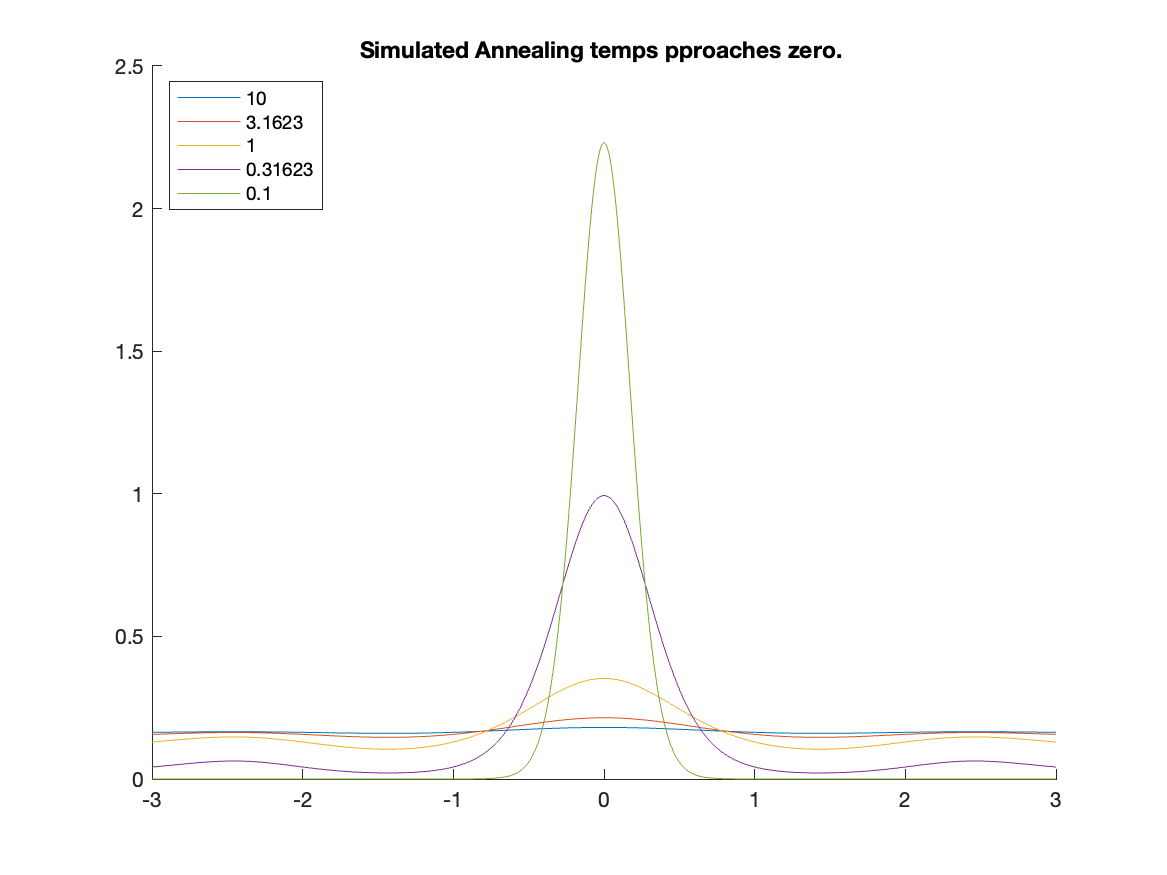
\includegraphics[width=14cm]{sa_temp.png}
            \caption{The distribution function of $\text{sinc}(x)$ as the temperature for simulated annealing gets smaller and smaller.}
            \label{fig:sa_temp}
        \end{figure}
        In practice, people use a function that controls the temperature for the SA to converge as the temperature gets lower and lower, which avoids exploring the whole landscape and wasting all the computing resources. Furthermore, to avoid the limitations of floating points, we consider a customized acceptance function for SA: 
        \begin{align*}
            \rho(x, y) := \min
            \left\lbrace
            \mathbbm 1 \{f(y) < f(x)\}\exp(f(y) - f(x)) + \mathbbm 1 \{f(y) \ge f(x)\}, 1
            \right\rbrace. 
        \end{align*}
\subsection{Solving the bin packing problem}
    The bin packing problem is an integer programming problem: 
    \begin{align*}
        \max \langle w, x\rangle \text{ s.t: } \langle w, x\rangle \le 1, x\in \{1, 0\}^n. 
    \end{align*}
    We look for a subset of numbers of the vector $w$ $1$ such that it sums up as close to one as possible while not exceeding one. This problem can be approached with SA. 
    \subsection{Best base chain to avoid the curse of dimensionality}
        The bin packing problem suffers from 
    \subsection{Numerical Experiments}

\appendix
\section{Bleeh Bleeh Bleeh I am not Listening}

\bibliographystyle{plain}
\bibliography{refs.bib}
\end{document}